\section{Fundamentals}
\label{sec:background-kdn}

\subsection{Knowledge-Defined Networking}
\label{subsec:background-kdn}
In 2003, D. Clark \textit{et al.} proposed a new construct, the Knowledge Plane (KP) \cite{clark_2003:knowledge_plane}, a distributed cognitive system additional to the traditional planes (data and control) of computer networks that permeates the network. This plane was proposed as a pervasive system that builds and maintains high-level models of what the network is supposed to do. KP was envisioned to rely on ML, aiming to bring many advantages to networking, such as automation (recognize-act) and recommendation (recognize-explain-suggest). Although, KP has the potential to represent a paradigm shift in the way the computer networks are operated, optimized, and troubleshot, up to now, such a plane has not been widely deployed. This constrained deployment is because of diverse shortcomings:

\begin{itemize}
    \item In traditional networks the learning is partial since the switches and routers only have a partial view and control, avoiding achieve a handle beyond local domain.
    \item Fifteen years ago, network devices located at DP had limited capabilities of storage and computing.
\end{itemize}{}

Nowadays, the shortcomings aforementioned may be overcome because, first, SDN provides a full control and rich view of the network from a logically centralized point. Second, the capabilities of network devices have significantly improved, facilitating the gather of information in real-time about packets and flow-granularity. Therefore, KDN has been proposed as a cooperative paradigm that applies ML to SDN \cite{mestres_2017:KDN}, aiming at learning the behavior of the network and, in some cases, automatically operate the network accordingly the learned. Furthermore, they corroborate the feasibility of using KDN for Routing in an Overlay Network and Resource Management in a Network Function Virtualization (NFV) scenario. To sum up, the final goal of KDN is to achieve self-driving networks. Figure~\ref{fig:kdn_architecture} depicts an overview of the KDN paradigm and its functional planes.

\begin{figure}[!ht]
    \centering
    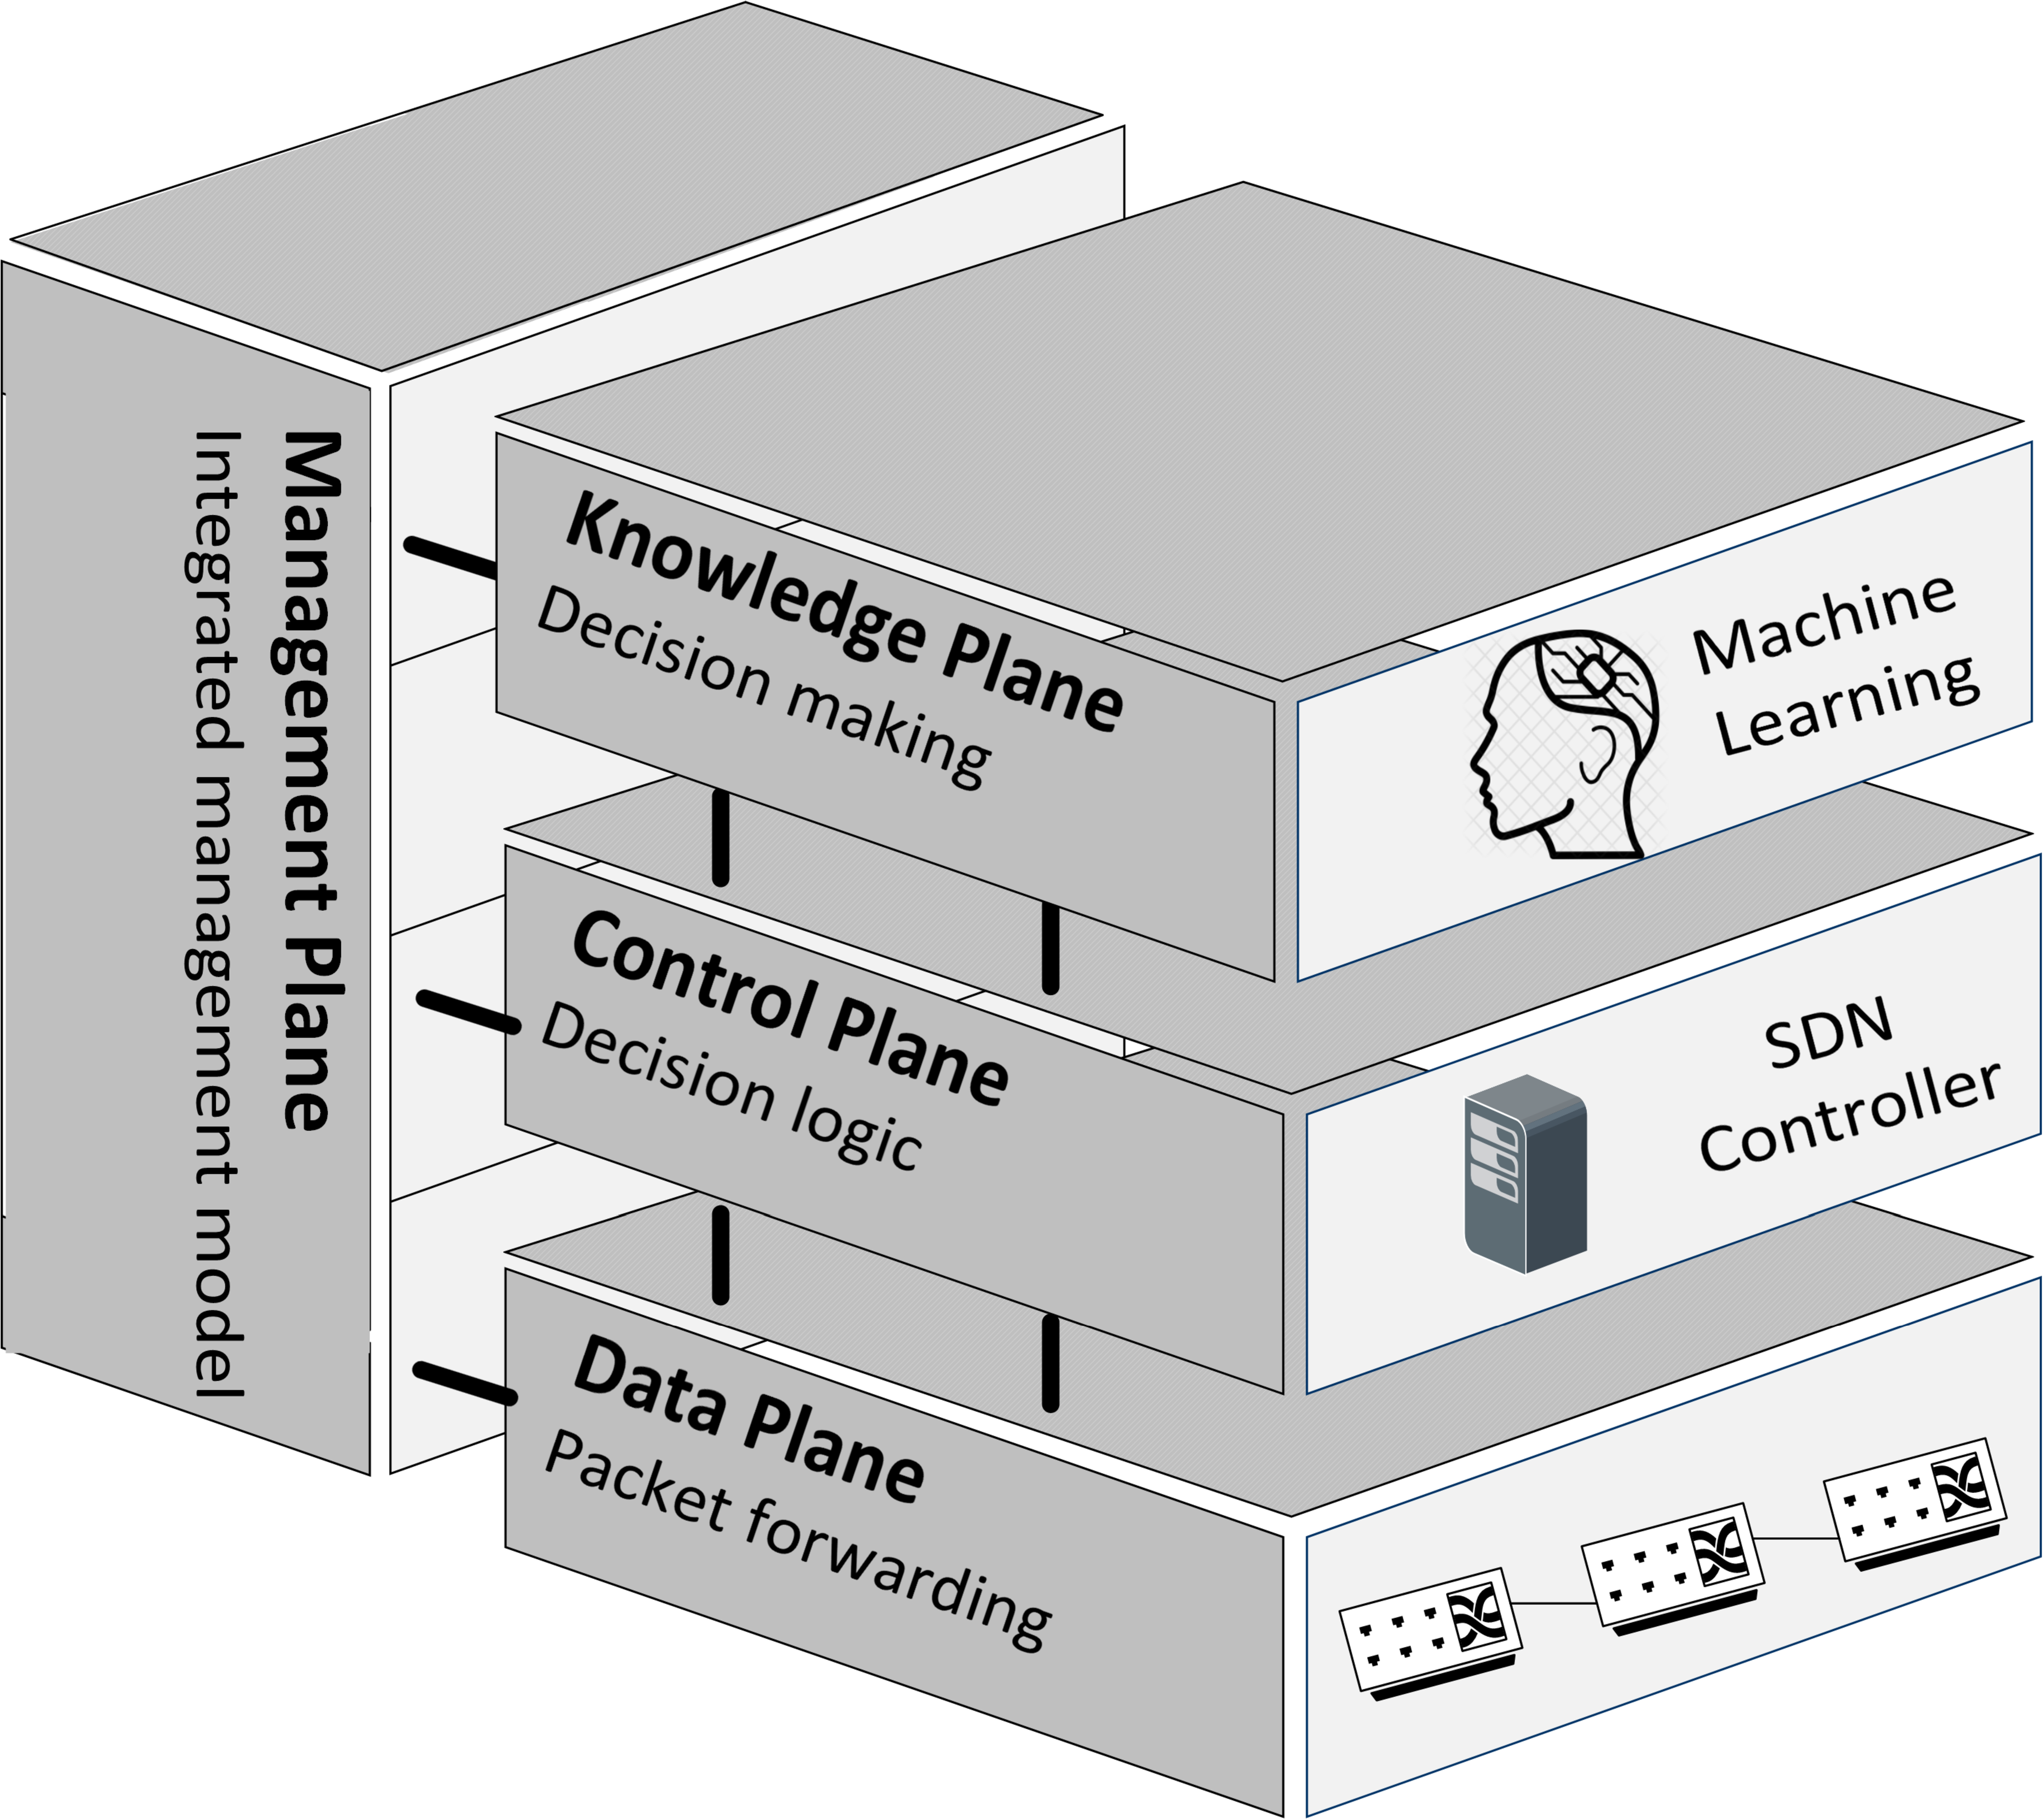
\includegraphics[scale=0.1]{figures/Figure1-KDN-architectured-3d.pdf}
    \caption{High-level KDN architecture (adapted from \cite{mestres_2017:KDN})}
    \label{fig:kdn_architecture}
\end{figure}

\begin{itemize}
    \item The DP is composed of network devices of programmable forwarding and is responsible for storing, forwarding and processing data packets. This plane depends on the CP and MP planes to populate the forwarding tables and update their configuration.
    
    \item The CP translates the requirements from the KP and AP in a specific network policy. Subsequently, CP is based on this policy to update and program matching and processing rules from the DP forwarding elements by SBI.
    
    \item The MP, as well as CP, ensures the correct operation and performance of the network in the long term. It defines the network topology and handles the provision and configuration of network devices. MP generates Metadata with information about the network state, events, statistical metrics per flow and per switch (\textit{e.g.}, packet loss, link failure, memory usage, and CPU utilization). The Metadata is sent to CP and KP. CP handles events that require immediate action (\textit{e.g.}, link failure, black-hole or loop detection). KP handles events that require knowledge (\textit{e.g.}, resource planning, optimization, performance management, and verification).
    
    \item The KP leverages MP and CP to obtain a rich view and control over the network. It is responsible for learning the behavior of the network and, in some cases, automatically operate the network accordingly. Fundamentally, the KP processes the Metadata generated by the MP, transforms them into knowledge via ML, and uses that knowledge to make decisions (either automatically or through human intervention). It is important to mention that, KP is separated from CP because ML algorithm is generally compute-intensive and it may affect the performance of the control plane.

\end{itemize}

This master dissertation supposes that RL is a technique useful to maintain MA and decrease the overhead of monitoring in SDN because it allows optimizing the probing interval by interacting with the network itself (\textit{i.e.,} environment in RL terms).\\

%It is to highlight that in \cite{mestres_2017:KDN}, the authors argue that KDN can be used to carry out intelligent network monitoring. It is because KDN would provide optimization, recommendation, and automation in the process of making decisions focused on improving the network behavior.
%\textbf{Knowledge-Defined Networking} encourages the use of ML to change the way the network operators handle, optimize and troubleshoot SDN \cite{mestres_2017:KDN}. In particular, By using ML techniques, it is possible to learn from the network behavior to provide automation (recognize-act) and recommendations (recognize-explain-suggest) that support management tasks. In turn, SDN offers full control and a network-wide view from a logically centralized point (\textit{i.e.}, controller). In this master dissertation, we argue that Reinforcement Learning (RL) is an ML technique useful to maintain MA and decrease the overhead of monitoring in SDN because it allows optimizing the probing interval by interacting with the network itself (\textit{i.e.,} environment in RL terms).

\subsection{Reinforcement Learning}
\label{subsec:background-rl}
In RL, an agent learns a decision-making process by interacting with an environment \cite{sutton_1998:rl}. Formally, in RL, the environment is typically modeled as a finite Markov Decision Processes (MDP) \cite{kolobov2012:markov} where the agent sends actions and receives outputs (observations and rewards). In a finite MDP, the agent and environment interact at discrete time steps $t = 0, 1, 2,..., N$. At each time-step $t$, the agent receives some representation of the state of the environment, ${S}_t \in S $, where $S$ is the set of possible states. Based on ${S}_t $, the agent selects an action, ${A}_t \in A(S_t) $, where $ A(S_t) $ is the set of available actions in the state ${S}_t $. The execution of action $A_{t}$ puts the agent into the new state $S_{t+1}$. Furthermore, the agent receives a numerical reward from the environment, $R_{t+1} \in  \mathbb{R}$ at step $t \in N$. Then, the total reward that the agent receives over its lifetime for this particular behavior is:

{\setlength{\mathindent}{6cm}
\begin{equation}
    \begin{split}
        U\left ( s \right ) = \sum_{t=0}^{\infty} \gamma^{t}R_{t}
    \end{split}
    \label{equ:total-reward}
\end{equation}
}
where $\gamma \in \left ( 0,1 \right ]$ is called the discount factor. If $\gamma < 1$, the discounting is used. Otherwise, it is not used. \\

RL algorithms find an optimal policy $ \Pi^{*}: S \rightarrow A $ that maximizes the expected cumulative reward for every state, using the exploration methods (\textit{e.g.}, $\varepsilon$-greedy, Boltzmann \cite{sutton_1998:rl} \cite{teng_2012:exploration}). The main RL features are its capacity to run without any prior knowledge of the environment (here, the monitored network) and make its own decisions in execution time (on-line). Nonetheless, RL requires a training period to capture the environment model before converging to the optimal policy.\\

\textbf{Q-learning} is one of the most important RL techniques \cite{duryea_2016:exploring_qlearning} because:

\begin{itemize}
    \item It was the pioneering RL method used for control purposes.
    \item It has a learning curve that tends to converge quickly.
    \item It is the simplest technique that directly calculates the optimal action policy without an intermediate cost evaluation step and without the use of a model \textit{(i.e.}, model-free).
    \item It has an off-policy learning capability; this means, the agent can learn an optimal policy (called Q-function), even if it does not always choose optimal actions. The only condition is that the agent regularly visits and updates all the $(S_t, A_t)$ pairs.
\end{itemize}{}

It is important to highlight that there are other RL strategies, such as Adaptive Heuristic Critic (AHC), Model-free Learning With Average Reward, and some Q-learning variations \cite{manju_2011:analysis_ql} \cite{kaelbling_1996:reinforcement}. These strategies are out of the scope of this master dissertation.\\

Q-learning \cite{Watkins:1989:q_learning} \cite{farahnakian_2011:q-learning} relies on an optimal action-value function $ Q_{t}(S_t,A_t)$, called Q-function. In this function, the value is the estimated reward of executing an action $A_t$ in the state $S_t$, assuming that the agent will follow the policy that provides the maximum reward. Q-learning starts with an arbitrary Q-function $Q_{0}$. At any state $S_{t}$, an agent selects an action $A_{t}$ that determines the transition to the next state $S_{t+1}$ and with the value associated to the pair ($S_t,A_t$) adjusts the values of Q-function according to:

{\setlength{\mathindent}{2cm}
\begin{equation}
    \begin{split}
        Q_{t+1}(S_t,A_t) \leftarrow & (1-\alpha) \cdot Q_{t}(S_t,A_t) + \alpha \cdot \left [R_{t+1} + \gamma \cdot \underset{\rm A}{\rm max} Q_{t}(S_{t+1},A) \right]
    \end{split}
    \label{equ:q_function}
\end{equation}
}

where $R_{t+1}$ denotes the reward received at time $t+ 1$, $\alpha \in \left [ 0,1 \right ]$ is the learning factor (a small positive number) that determines the importance of the acquired reward. A factor $\alpha = 0$ makes the agent does not learn from the latest ($S_t,A_t$) pair. In turn, a factor $\alpha = 1$ makes the agent considers the immediate rewards without taking into account the future rewards. $\gamma \in \left [ 0,1 \right ]$ is the discount factor that determines the importance of future rewards. A factor $\gamma = 0$ prohibits the agent from acquiring future rewards. A factor $\gamma = 1$ forces the agent only to consider future rewards. The part between square brackets is the updated value that represents the difference between the current estimate of the optimal Q-value $Q_t(S_t,A_t)$ for a state-action pair ($  S_{t}, A_{t} $), and the new estimate $ \left [R_{t+1} + \gamma  \underset{\rm A}{\rm max} Q_t(S_{t+1},A) \right ]$.\\

The Q-function approximates the optimal state-action value function $ Q^*$ regardless of the followed policy. It is noteworthy that the updated Q-function $Q_{t} $ only depends on the previous function $Q_{t-1} $ combined with the experience ($S_{t}, A_{t}, R_{t}, S_{t+1}$). Thus, Q-learning is both computationally and memory efficient. Nonetheless, if the number of states is high, Q-learning may take much time and require more data to converge (\textit{i.e.,} find the best action for each state). Therefore, in Q-learning is critical to have a concise representation of the environment (\textit{i.e.,} the network model).\\

To find the Q-function, Q-learning requires an exploration method. The exploration method selects an action to perform at each step, which represents the Q-function. $\varepsilon$-greedy exploration is one of the most used exploration methods \cite{teng_2012:exploration} \cite{Tijsma_2016:exploration_q_learning}. It uses $\varepsilon \in \left [ 0,1 \right ]$ as the parameter of exploration to decide which action to perform using $Q_{t}(S_{t},A)$. With this parameter the action is as follows:

{\setlength{\mathindent}{4cm}
\begin{equation}
    \begin{split}
       \mathcal{A} = \begin{Bmatrix}
            \underset{\rm A}{\rm max} Q_{t}(S_{t},A) & with \thinspace probability\thinspace 1-\varepsilon \\ 
            random\thinspace action & with\thinspace probability \thinspace \varepsilon
        \end{Bmatrix}
    \end{split}
    \label{equ:e-greedy}
\end{equation}
}

$\varepsilon$-greedy exploration method adds some randomness when deciding between actions. Instead of always selecting the best available action, this method randomly explores other actions with a probability = $\varepsilon$ or chooses the best action (highest Q-value) with a probability = $1-\varepsilon$. A high value for $\varepsilon$ adds randomness to the exploration method, which will make the agent explores other actions more frequently. Randomness is necessary for an agent to learn the optimal policy.